\documentclass{handout}

% \SetInstructor{Lt Col James Phillips}
\SetCourseTitle{ECE231: Electrical Circuits and Systems I}
\SetSemester{Fall 2016}
\SetHandoutTitle{Lecture 30: Phasors Circuit Analysis and Design Part 2}

%\SetDueDate{1 Jan 2016}
%\ShowAllBlanks

\showsoln \setsolncolor{red}

\begin{document}
\maketitle

\textbf{OBJECTIVES:}
\begin{enumerate}
\item Learn to apply circuit analysis techniques we already know to solve circuits in the phasor domain
\end{enumerate}

\textbf{READING}
\begin{description}
\item [Required]:
Textbook, section 8.4--8.5, pages 402--426
\item [Optional]:
\end{description}

\section{Introduction}
Today we continue our analysis of phasor circuits.  Last class we did examples of:
\begin{enumerate}
\item Parallel and series combinations of \textbf{Impedances}
\item Voltage and Current Division
\item Mesh and Node Analyisis
\end{enumerate}

Today we will look at:
\begin{enumerate}
\item Proportionality and Superposition
\item Thevenin and Norton equivalent circuits
\end{enumerate}

All these things still apply to phasor domain circuits. As a reminder, phasor analysis only applies to the steady state sinusoidal responses.  Phasor analysis does not tell you anything about the transient response.


\section{Proportionality}
Back in lesson 8 we introduced this introduced this idea of proportionality which states that for a linear circuit, any change to the input has a proportional change to the output.  Stated mathematically:
\[
y=Kx
\]
where $x$ is the input, $y$ is the output, and $K$ is the proportionality factor.

This also applies to phasors and can be written as:
\[
\mathbf{Y} = \mathbf{KX}
\]
where $Y$, $X$, and $K$ are all in general complex.

To make use of proportionality, the book talks about the {\em Unit Output Method}.... I prefer the {\em Unit Input Method}.  Let's do an example:

\textbf{Example 1}-- This example is a modified version of textbook exercise 8-22.  For the circuit shown in Figure \ref{fig: Example1}, use the Unit Input Method to find $\mathbf{I_o}$

\begin{figure} [h!]
\centering
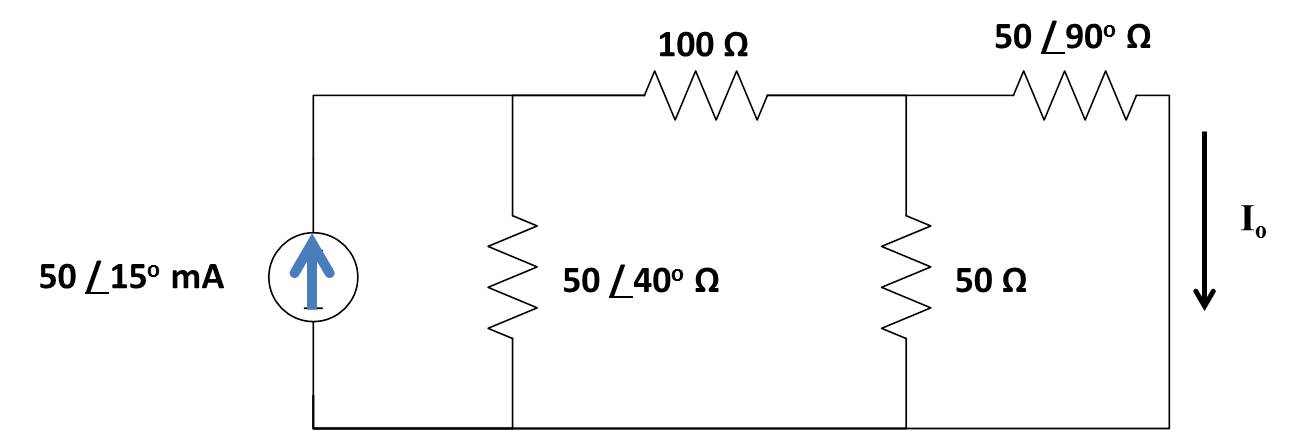
\includegraphics[width=0.5\textwidth]{Example1.jpg}
\caption{Circuit to accompany example 1}
\label{fig: Example1}
\end{figure}


\soln{4in}{
\begin{figure} [h!]
\centering
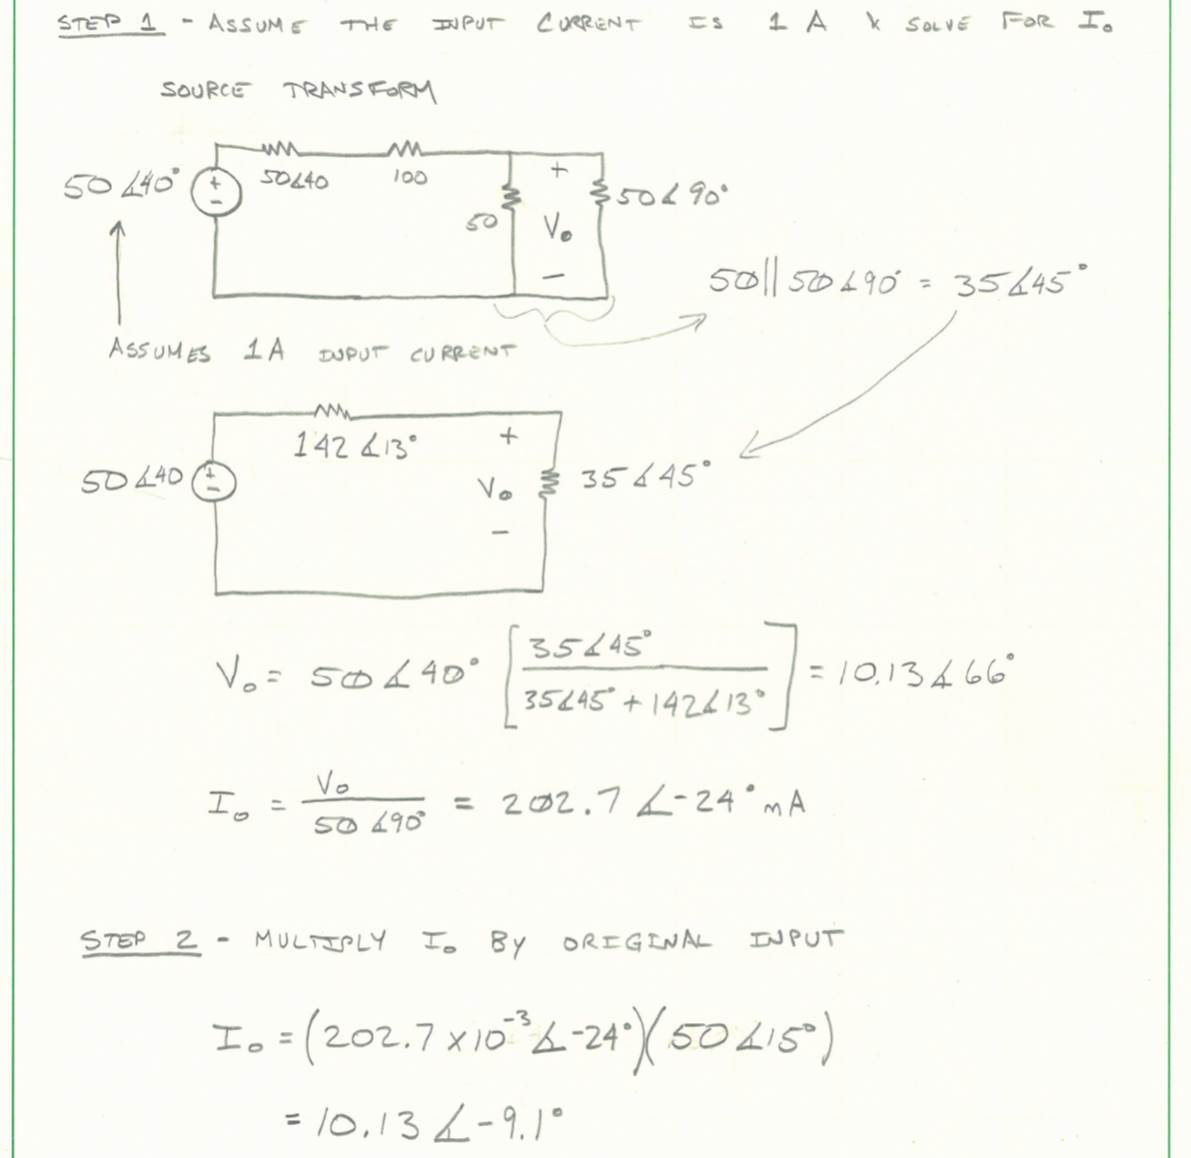
\includegraphics[width=0.6\textwidth]{Example1soln.jpg}
\end{figure}
}


\newpage
\clearpage
\pagebreak

\section{Superposition}
Before we jump right into an example, now is a good opportunity to remind you that phasor analysis only works for circuits that are excited by a single sinusoidal frequency.  This does not mean we cannot have more than one source, it just means they all have to have the same frequency ($\omega$).

\textbf{Example 2} -- Textbook Exercise 8-23 --- For the circuit in Figure \ref{fig: Example2}, use superposition to find $\mathbf{I_x}$.
\begin{figure} [h!]
\centering
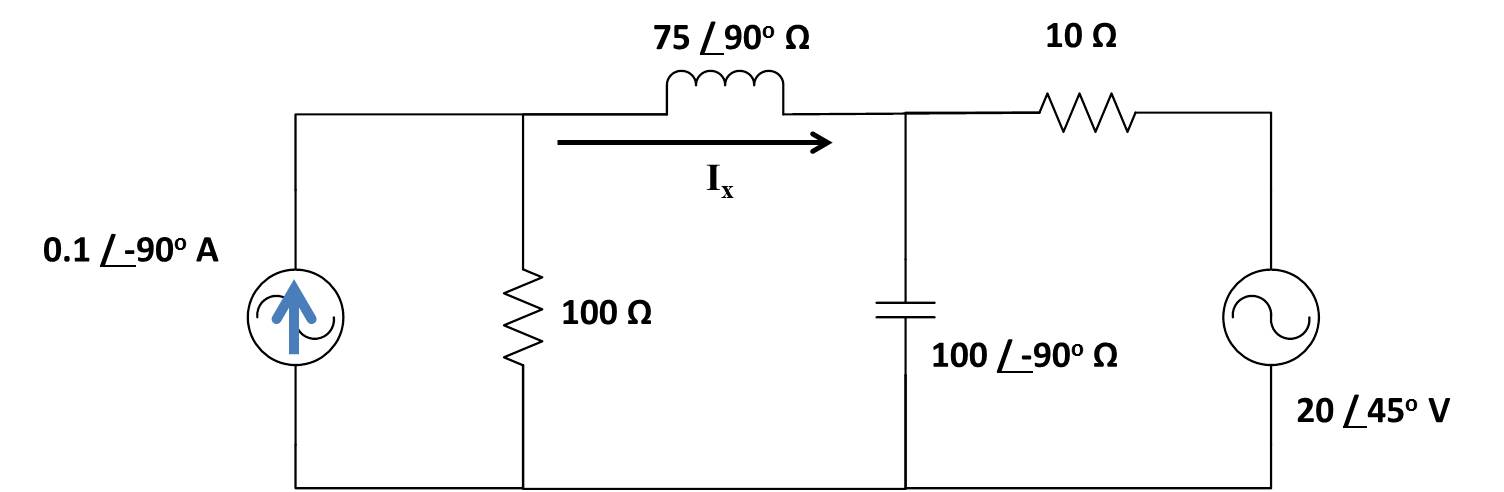
\includegraphics[width=0.7\textwidth]{Example2.jpg}
\caption{Circuit to accompany example 2}
\label{fig: Example2}
\end{figure}

\soln{4in}{
\begin{figure} [h!]
\centering
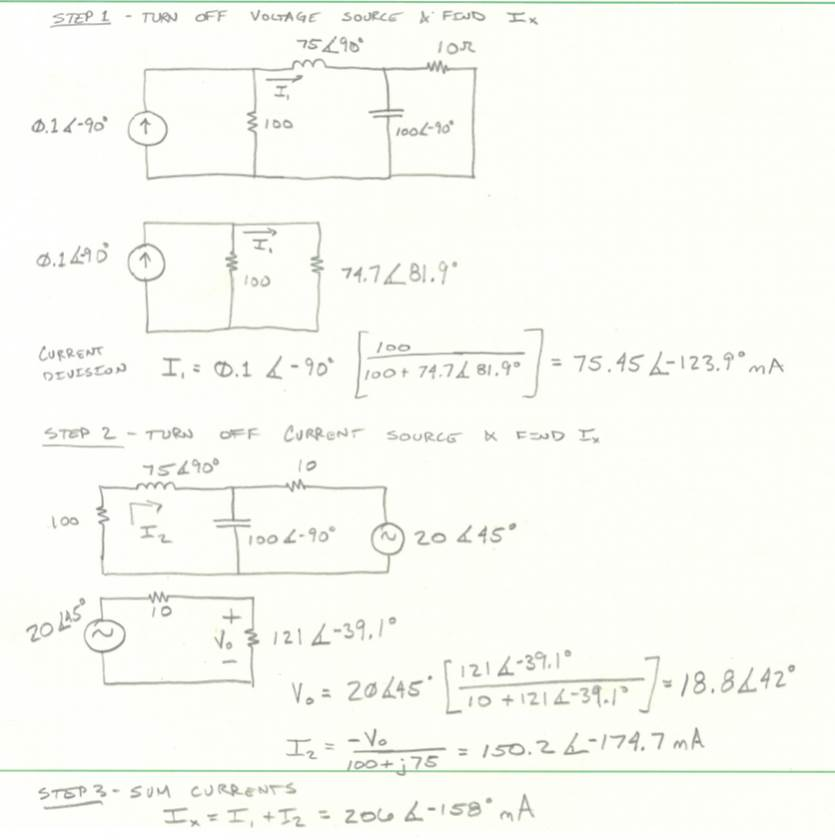
\includegraphics[width=0.85\textwidth]{Example2soln.jpg}
\end{figure}
}

\newpage
\clearpage
\pagebreak

\section{Thevenin's and Norton's Theorems}
This section will offer a quick review of Thevenin's and Norton's Theorems before we work a couple of examples.

For Thevenins theorem, we will take a {\em source} circuit that is connected to some {\em load} circuit and replace the source circuit with a single voltage source in series with a single {\em impedance}.  To do this we must find the value of the source voltage and the {\em Thevenin impedance}.  The source voltage is found by calculating the open circuit voltage if the load is removed.  The easiest way to calculate the Thevenin Impedance is by using look-back.

 \textbf{Example  3}-- Textbook Exercise 8-29 --- For the curcuit in example 2 (Figure \ref{fig: Example2}), find the  Thevenin circuit seen by the inductor then calculate $\mathbf{I_X}$.

\soln{6in}{
\begin{figure} [h!]
\centering
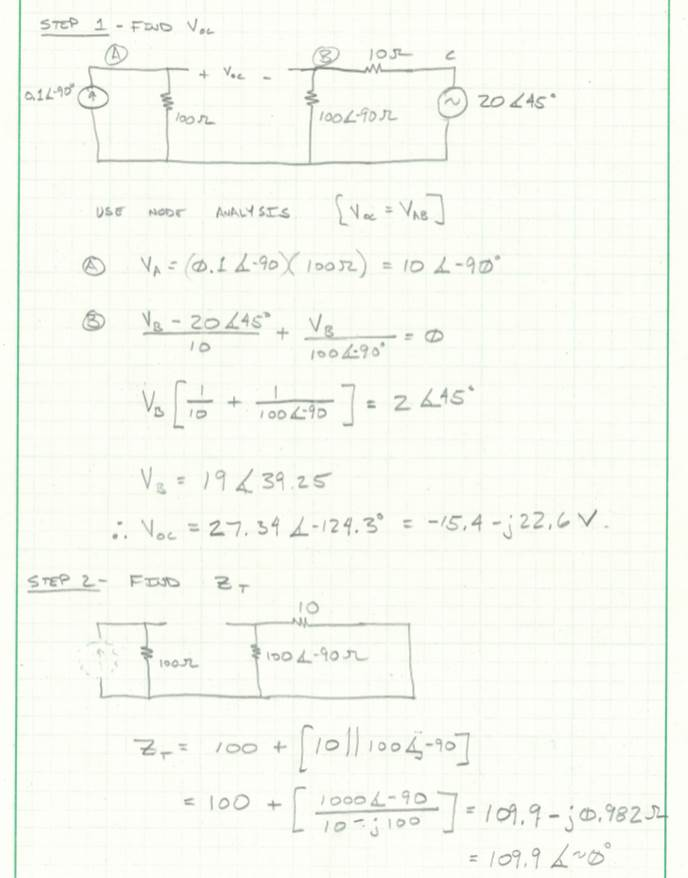
\includegraphics[width=0.8\textwidth]{Example3solnA.jpg}
\end{figure}

\begin{figure} [h!]
\centering
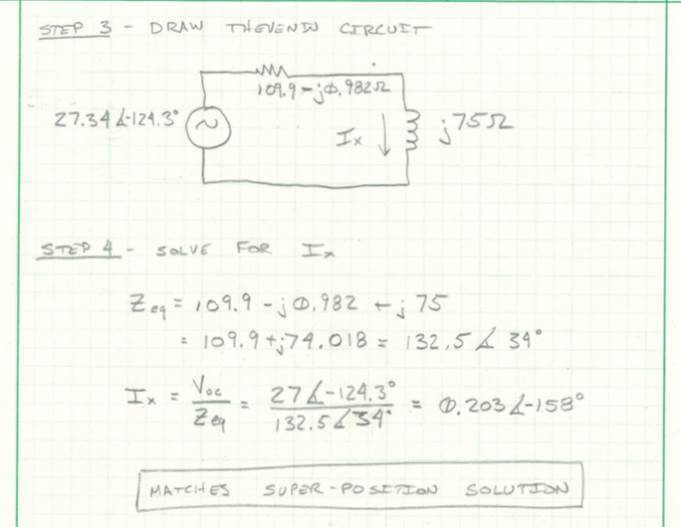
\includegraphics[width=1\textwidth]{Example3solnB.jpg}
\end{figure}
}

\newpage
\clearpage
\pagebreak

Norton's Theorem is like Thevenin's except we find a current source in parallel with an impedance.

\textbf{Example 4} -- Rework Example 3 with Norton's Theorem.

\soln{6in}{
\begin{figure} [h!]
\centering
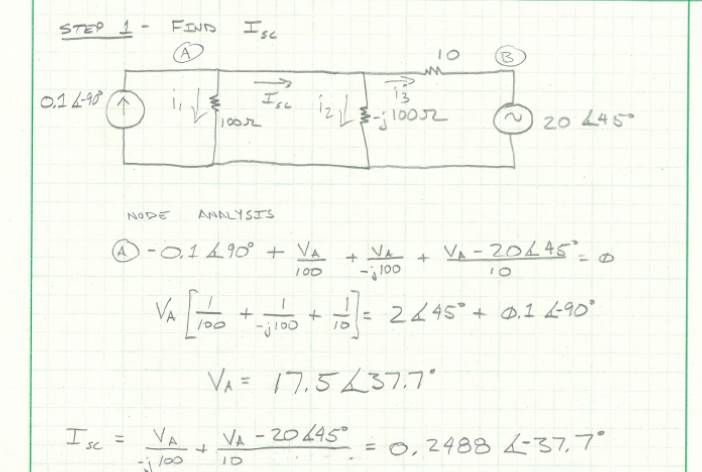
\includegraphics[width=1\textwidth]{Example4solnA.jpg}
\end{figure}

\begin{figure} [h!]
\centering
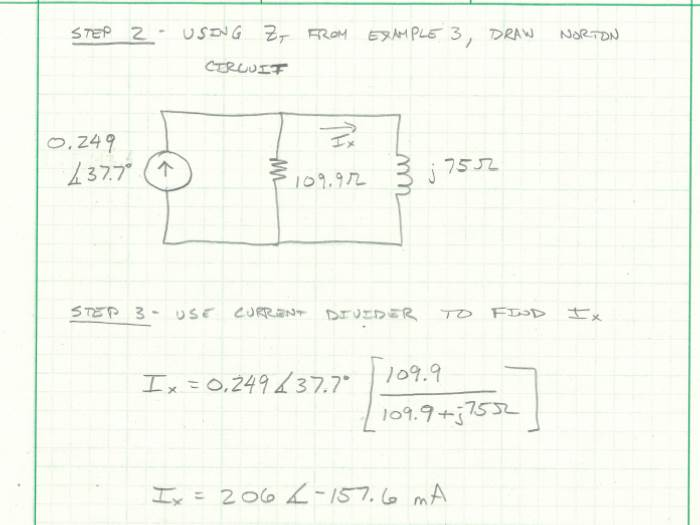
\includegraphics[width=1\textwidth]{Example4solnB.jpg}
\end{figure}
}

\newpage
\clearpage
\pagebreak

\newpage
\clearpage
\pagebreak

\newpage
\clearpage
\pagebreak




\end{document}


% Equation Array Example Code
%\begin
%{eqnarray}
%P_R &=& i_R^2R \nonumber \\
%P_R &=& (100\ mA)^2 \times 100\ \Omega \nonumber \\
%P_R &=& (100 \times 10^{-3}\ A)^2 \times 100\ \Omega \\
%P_R &=& 10000 \times 10^{-6}\ A^2  \times 100\ \Omega \nonumber \\
%P_R &=& 1\ W  \nonumber
%\end{eqnarray}

% Figure Example Code
%\begin{figure} [h!]
%\centering
%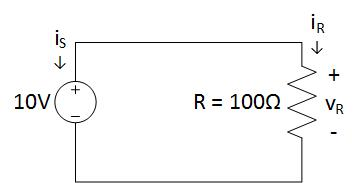
\includegraphics[width=0.5\textwidth]{OhmsLawExampleSolution.jpg}
%\caption{Ohm's Law example circuit}
%\label{fig: OhmsLawExampleSolution}
%\end{figure}

%Table Example Code
%\begin{table}[h]
%\centering
%\begin{tabular}{|l|c|c|}
%\hline
%Prefix & Abbreviation & Value \\
%\hline \hline
%Giga & $G$ & $10^9$ \\
%Mega & $M$ & $10^6$ \\
%Kilo & $k$ & $10^3$ \\
%\hline
%milli & $m$ & $10^{-3}$ \\
%micro & $\mu$ & $10^{-6}$ \\
%nano & $n$ & $10^{-9}$ \\
%pico & $p$ & $10^{-12}$ \\
%\hline
%\end{tabular}
%\caption{Engineering prefixes and values}
%\label{tab: Eng Prefixes}
%\end{table}
